\documentclass{article}
\usepackage{amsmath,amssymb}
\usepackage{tikz}
\usetikzlibrary{calc}

\begin{document}

\section*{What is Fisher information?}

\[
I(\theta) \;=\; \mathbb{E}\!\Biggl[\Bigl(\tfrac{\partial}{\partial \theta}\ln f(Y;\theta)\Bigr)^{2}\Biggr].
\]

\subsection*{Example: \(Y = \theta + W\), \(W \sim \mathcal{N}(0,\sigma^{2})\)}

\[
f(y;\theta)
\;=\;
\frac{1}{\sqrt{2\pi}\,\sigma}
\exp\!\Bigl(-\tfrac{(y-\theta)^{2}}{2\sigma^{2}}\Bigr).
\]

\noindent
The Fisher information is then found by
\[
I(\theta)
\;=\;
\int_{-\infty}^{\infty}
f(y;\theta)\,
\biggl(
  \tfrac{\partial}{\partial \theta}
  \ln f(y;\theta)
\biggr)^{2}
\,dy
\;=\;
\frac{1}{\sigma^{2}}.
\]

\subsection*{Block diagram (schematic)}

\begin{center}
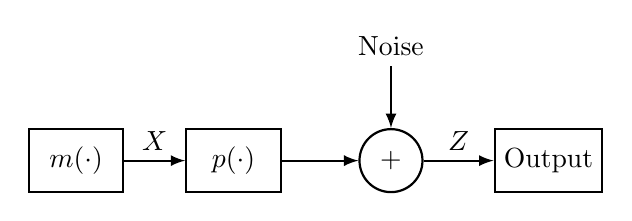
\begin{tikzpicture}[>=latex,thick,node distance=2.0cm]
  \node[draw, rectangle, minimum width=1.2cm, minimum height=0.8cm] (m) {$m(\cdot)$};
  \node[draw, rectangle, right of=m, minimum width=1.2cm, minimum height=0.8cm] (p) {$p(\cdot)$};
  \node[circle, draw, right of=p, minimum size=0.8cm, node distance=2cm] (plus) {$+$};
  \node[draw, rectangle, right of=plus, minimum width=1.2cm, minimum height=0.8cm, node distance=2cm] (out) {Output};

  \draw[->] (m) -- (p) node[midway, above] {$X$};
  \draw[->] (p) -- (plus) node[midway, above] {};
  \draw[->] (plus) -- (out) node[midway, above] {$Z$};
  \draw[->] ($(plus)+(0,1.2)$) node[above] {Noise} -- (plus);
\end{tikzpicture}
\end{center}

\end{document}

